\documentclass{article}
\usepackage{tkz-euclide}
\usepackage{tikz}
\usepackage{tikz-3dplot}
\usetikzlibrary{fit}

\begin{document}

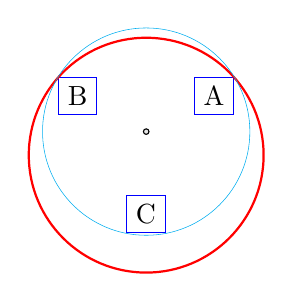
\begin{tikzpicture}
\node[draw=blue] (A) at (30:1cm) {A};
\node[draw=blue] (B) at (150:1cm) {B};
\node[draw=blue] (C) at (270:1cm) {C};

\node[circle,draw=red,thick,fit=(A) (B) (C),inner sep=0pt] {};

\coordinate (a) at (A.north east);
\coordinate (b) at (B.north west);
\coordinate (c) at (C.south east);
\tkzCircumCenter(a,b,c)
\tkzGetPoint{O}
\tkzDrawPoint(O)
\tkzDrawCircle[color=cyan](O,a)
\end{tikzpicture}

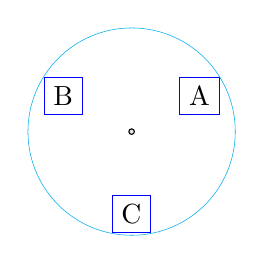
\begin{tikzpicture}
\node[draw=blue] (A) at (30:1cm) {A};
\node[draw=blue] (B) at (150:1cm) {B};
\node[draw=blue] (C) at (270:1cm) {C};

%\node[circle,draw=red,thick,fit=(A) (B) (C),inner sep=0pt] {};

\coordinate (a) at (A.north east);
\coordinate (b) at (B.north west);
\coordinate (c) at (C.south east);

\tkzCircumCenter(a,b,c)
\tkzGetPoint{O}
\tkzDrawPoint(O)
\tkzDrawCircle[color=cyan](O,a)
\end{tikzpicture}




\tdplotsetmaincoords{70}{110}
\begin{tikzpicture}[tdplot_main_coords]
\draw[thick,->] (0,0,0) -- (6,0,0) node[anchor=north east]{$x$};
\draw[thick,->] (0,0,0) -- (0,4,0) node[anchor=north west]{$y$};
\draw[thick,->] (0,0,0) -- (0,0,3) node[anchor=south]{$z$};
\pgfmathsetmacro{\ax}{1}
\pgfmathsetmacro{\ay}{1}
\pgfmathsetmacro{\az}{1}
\draw[->,red] (0,0,0) -- (\ax,\ay,\az);
%\draw[dashed,red] (0,0,0) -- (\ax,\ay,0) -- (\ax,\ay,\az);
\tdplotgetpolarcoords{\ax}{\ay}{\az}
\tdplotsetthetaplanecoords{\tdplotresphi}
\tdplotdrawarc[tdplot_rotated_coords]{(0,0,0)}{1}{0}
{\tdplotrestheta}{anchor=west}{$\theta = \tdplotrestheta$}

\node (A) at (0:2cm) {A};
\node (B) at (90:2cm) {B};
\node (C) at (225:2cm) {C};


\coordinate (a) at (A.north east);
\coordinate (b) at (B.north west);
\coordinate (c) at (C.south east);

\tkzCircumCenter(a,b,c)
\tkzGetPoint{O}
%\tkzDrawPoint(O)
\tkzDrawCircle[color=cyan](O,a)


\end{tikzpicture}





\tdplotsetmaincoords{70}{110}
\begin{tikzpicture}[tdplot_main_coords]
\draw[thick,->] (0,0,0) -- (6,0,0) node[anchor=north east]{$x$};
\draw[thick,->] (0,0,0) -- (0,4,0) node[anchor=north west]{$y$};
\draw[thick,->] (0,0,0) -- (0,0,3) node[anchor=south]{$z$};
\pgfmathsetmacro{\ax}{1}
\pgfmathsetmacro{\ay}{1}
\pgfmathsetmacro{\az}{1}
\draw[->,red] (0,0,0) -- (\ax,\ay,\az);
%\draw[dashed,red] (0,0,0) -- (\ax,\ay,0) -- (\ax,\ay,\az);
\tdplotgetpolarcoords{\ax}{\ay}{\az}
\tdplotsetthetaplanecoords{\tdplotresphi}
\tdplotdrawarc[tdplot_rotated_coords]{(0,0,0)}{1}{0}
{\tdplotrestheta}{anchor=west}{$\theta = \tdplotrestheta$}

\node (A) at (0:2cm) {};
\node (B) at (90:2cm) {};
\node (C) at (225:2cm) {};


\coordinate (a) at (A.north east);
\coordinate (b) at (B.north west);
\coordinate (c) at (C.south east);

\tkzCircumCenter(a,b,c)
\tkzGetPoint{O}
%\tkzDrawPoint(O)
\tkzDrawCircle[color=cyan](O,a)


\end{tikzpicture}










\end{document}